\documentclass[conference]{IEEEtran}
\IEEEoverridecommandlockouts
% The preceding line is only needed to identify funding in the first footnote. If that is unneeded, please comment it out.
%Template version as of 6/27/2024

\usepackage{cite}
\usepackage[most]{tcolorbox}
\usepackage{amsmath,amssymb,amsfonts}
\usepackage{algorithmic}
\usepackage{graphicx}
\usepackage{textcomp}
\usepackage{xcolor}
\usepackage{float}
\def\BibTeX{{\rm B\kern-.05em{\sc i\kern-.025em b}\kern-.08em
    T\kern-.1667em\lower.7ex\hbox{E}\kern-.125emX}}
\begin{document}

\title{Model simulation of an orbit with an internally moving mass\\
}

\author{
\IEEEauthorblockN{Lukas Ehlers} \\
\IEEEauthorblockA{\textit{UiT The Arctic University of Norway} \\
\textit{Department of Computer Science} \\
Tromsø, Norway }
}

\maketitle

\begin{abstract}
This study explores the impact of internal mass shifts on the orbital dynamics of a satellite in a gravitational field. Using a simplified model with a movable inner mass, the research examines how such shifts, driven by a solar-powered electric motor, influence the satellite's trajectory over time. The results show that even small changes in mass distribution can lead to significant alterations in the orbit, offering insights for satellite systems with movable internal components. Numerical simulations based on Newton’s law of gravitation and the Runge-Kutta method are used to track the satellite's motion and demonstrate the long-term effects of these mass displacements.
\end{abstract}

\begin{IEEEkeywords}
    todo,todo
\end{IEEEkeywords}

\section{Einleitung}

The lifespan of modern satellites is largely determined by the amount of fuel available. This fuel is not only required for orbital maneuvers and course corrections but is often also used for stabilization and attitude control. Once the fuel is depleted, operational activity often ceases, even though all other systems may still be fully functional.

Against this backdrop, alternative methods are being explored to achieve control or orbit-modifying effects without active fuel consumption. One promising idea is to deliberately use internal mass shifts to influence a satellite’s orbit or orientation through inertia and gravitational effects. This study investigates how the position of a movable internal mass affects the orbit of a body within the gravitational field of a central body.

\section{Theoretische Grundlagen}

The physical foundation of this study is based on several fundamental principles of classical mechanics. First, in a closed system with no external forces, the law of conservation of momentum applies: the total momentum remains constant, even when masses move within the system \cite{goldstein}. This means that shifting an internal mass — for example, via an electric motor inside a cylinder — does not change the system’s overall center of mass as long as no external force is acting on it.

Moreover, the center of mass of an extended body in a gravitational field moves as if the entire mass were concentrated at that point \cite{taylor, landau}. This allows the trajectory of the system to be calculated without directly considering the internal mass distribution, as long as the external field can be approximately treated as central.

A key result is that internal mass shifts do not affect the orbit of a closed system in a gravitational field, but can only alter its rotational dynamics. This is well known in aerospace engineering, for example in satellites equipped with reaction wheels or movable fuel tanks \cite{marion}.

Finally, Noether’s theorem provides a deeper theoretical foundation: it establishes the connection between symmetries and conserved quantities. For instance, translational symmetry leads to momentum conservation, while rotational symmetry leads to the conservation of angular momentum \cite{noether}.




\section{Gravitationskraft}

The gravitational force on an object with mass \( m \) in the field of a central body with mass \( M \) is given by:

\[
\vec{F}_\text{grav} = -G \cdot \frac{M \cdot m}{r^2} \cdot \hat{r}
\]

Where:
\begin{itemize}
  \item \( G \): Gravitational constant
  \item \( M \): Mass of the central body
  \item \( m \): Mass of the orbiting body (cylinder + weight)
  \item \( r \): Distance between the center of mass of the body and the center of the central body
  \item \( \hat{r} \): Unit vector pointing from the body’s center of mass to the central body
\end{itemize}


\section{Ansatz bewegliches Gewicht}

\begin{figure}
    \centering
    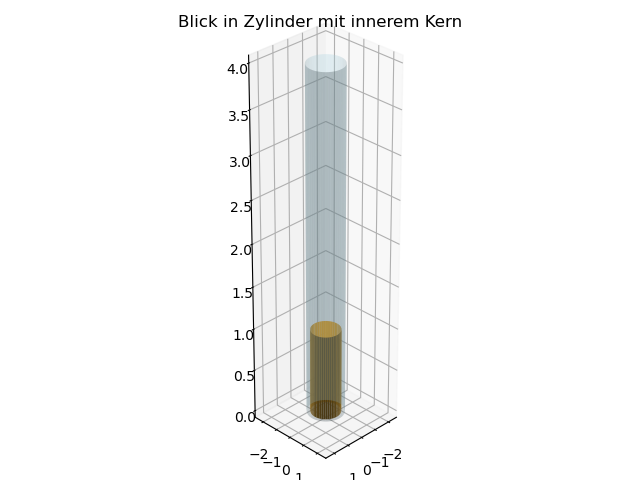
\includegraphics[width=\linewidth]{pics/sat_model_abstract/plot.png}
    \caption{Model bewegliches Gewicht}
    \label{fig:abstract_model}
\end{figure}


Figure~\ref{fig:abstract_model} shows a simplified model of a rotationally symmetric body, consisting of a larger outer cylinder that contains a smaller, movable inner cylinder. The schematic representation includes only the basic geometric structures. The technical mechanism for shifting the internal mass is not shown: the inner cylinder is mounted on a threaded shaft and can be moved along the cylinder axis. The displacement is driven by a compact electric motor that operates without conventional fuel. Instead, the motor is powered solely by solar energy, which is captured by solar panels mounted on the outer cylinder and converted into electrical energy.


\section{Schwerpunkt des Systems}
The complete system consists of:
\begin{itemize}
  \item Cylindrical shell with mass \( m_\text{body} = 9 \)
  \item Movable weight with mass \( m_\text{payload} = 1 \)
\end{itemize}

The position of the center of mass is given by:

\[
\vec{r}_\text{cm} = \frac{m_\text{body} \cdot \vec{r}_\text{body} + m_\text{payload} \cdot \vec{r}_\text{payload}}{m_\text{body} + m_\text{payload}}
\]

\subsection*{Fall: Gewicht weiter entfernt vom Planeten}

Given:
\[
\vec{r}_\text{body} = (10, 0), \quad \vec{r}_\text{payload} = (11, 0)
\]

Required:
\[
\vec{r}_\text{cm} = \frac{9 \cdot (10, 0) + 1 \cdot (11, 0)}{10} = (10.1, 0)
\]

\section{Gravitationskraft auf den Schwerpunkt}

Central mass: \( M = 1000 \), total mass: \( m = 10 \), distance: \( r = 10.1 \), Gravitational constant: \( G = 1 \)

\[
\vec{F} = - G \cdot \frac{M \cdot m}{r^2} \cdot \frac{\vec{r}_\text{cm}}{r}
= - \frac{1000 \cdot 10}{10.1^2} \cdot \frac{(10.1, 0)}{10.1}
\]

\[
= - \frac{10000}{102.01} \cdot (1, 0) \approx -98.03 \cdot (1, 0) = (-98.03, 0)
\]

\section{Beschleunigung}

\[
\vec{a} = \frac{\vec{F}}{m} = \frac{(-98.03, 0)}{10} = (-9.803, 0)
\]

\section{Numerische Integration (Euler-Verfahren)}

\begin{align*}
\vec{v}_\text{neu} &= \vec{v} + \vec{a} \cdot \Delta t = (0, 3.0) + (-9.803, 0) \cdot 0.01  \\
\vec{v}_\text{neu} &= (-0.098, 3.0) \\
\vec{r}_\text{neu} &= \vec{r} + \vec{v}_\text{neu} \cdot \Delta t = (10.0, 0.0) + (-0.098, 3.0) \cdot 0.01 \\
\vec{r}_\text{neu} &=(9.99902, 0.03)
\end{align*}


\section{Simulation}

\begin{figure}[H]
    \centering
    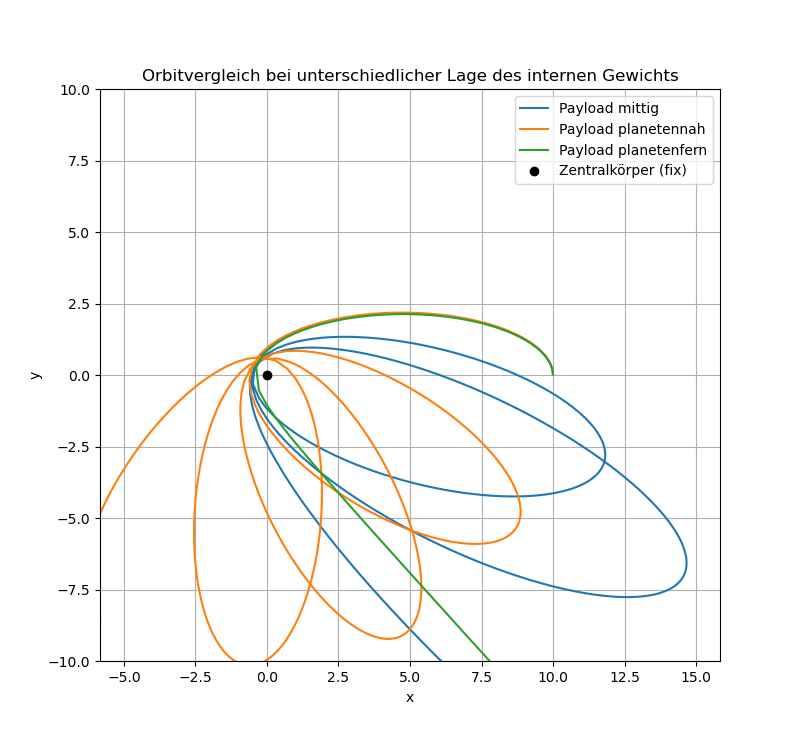
\includegraphics[width=\linewidth]{pics/orbits.png}
    \caption{unterschiedliche Orbits je nach Lage der Masse}
    \label{fig:orbits}
\end{figure}

The trajectories shown in Figure~\ref{fig:orbits} clearly demonstrate that the orbit of the body changes slightly depending on the position of the internal mass. Although the total mass of the system remains unchanged, the shift in the center of mass leads to altered initial accelerations, and consequently, to different orbital paths.

The most noticeable orbit is the one with the weight near the planet (orange curve): it exhibits stronger orbital curvatures, which can be attributed to higher gravitational accelerations with a closer center of mass. The orbit appears more unstable and oscillates more, which over longer periods can lead to a noticeably different orbital dynamics.

In contrast, the green curve (weight far from the planet) shows a slightly flatter and more stable orbit with a larger apogee. The center of mass is farther from the central body, reducing the gravitational force and thus widening the orbit.

The middle configuration (blue) serves as a reference. It shows a more symmetric orbit, as the center of mass of the system coincides with the geometric center of the cylinder.

These results demonstrate that even small variations in the internal mass distribution can lead to significant long-term differences in the motion, which is particularly important for precise navigation or orbit control — such as in satellites with movable internal mass (e.g., fuel shifting, mobile payloads).


\subsection{Numerische Simulation der Satellitenbewegung}
-LINK ZU GITHUB MIT CODE-

The simulation of the satellite motion is based on Newton's law of gravitation, which determines the gravitational force between the Earth and the satellite. To integrate the motion over time, the classical Runge-Kutta method is used, which is known for its high accuracy in numerically calculating position and velocity. In each time step, the current position and velocity values of the satellite are updated using this method, so that over time an orbit is generated, which is then visualized.


\section{Analysis of Center of Mass and Angular Momentum Changes due to Internal Mass Redistribution}

\subsection{Given Constants}

\begin{itemize}
  \item \( G \): Gravitational constant
  \item \( M \): Mass of Earth
  \item \( m_\text{sat} \): Mass of the satellite body
  \item \( m_\text{payload} \): Mass of the movable internal weight
  \item \( r \): Mean distance to Earth's center
  \item \( L \): Length of the internal tube
  \item \( T \): Orbital period
\end{itemize}


\begin{align*}
G &= 6.67430 \times 10^{-11} \; \text{m}^3\,\text{kg}^{-1}\,\text{s}^{-2} \\
M &= 5.972 \times 10^{24} \; \text{kg}  \\
m_\text{sat} &= 1 \; \text{kg}  \\
m_\text{payload} &= 1 \; \text{kg} \\
r &= 7.0 \times 10^6 \; \text{m}  \\
L &= 2.0 \; \text{m}  \\
T &= 5400 \; \text{s} && \text{(90 minutes)}
\end{align*}

\subsection{Orbital Speed}
The orbital speed $v$ at a circular orbit is computed by:
\[
v = \sqrt{\frac{GM}{r}} = \sqrt{\frac{6.67430 \times 10^{-11} \cdot 5.972 \times 10^{24}}{7.0 \times 10^6}} \approx 7546 \; \text{m/s}
\]

\subsection{Computation of Center of Mass}
Assuming the satellite mass is $m_\text{sat}$ and the payload can move along the radial direction with offset $\Delta r$, the center of mass becomes:
\[
r_\text{com} = \frac{m_\text{sat} \cdot r + m_\text{payload} \cdot (r + \Delta r)}{m_\text{sat} + m_\text{payload}}
\]

We evaluate for three positions:

\begin{itemize}
  \item \textbf{Payload at the bottom} ($\Delta r = -1.0 \, \text{m}$):
  \[
  r_\text{com} = \frac{7.0 \times 10^6 + (7.0 \times 10^6 - 1)}{2} = 3,499,999.5 \; \text{m}
  \]
  The center of mass is slightly closer to Earth.

  \item \textbf{Payload centered} ($\Delta r = 0.0 \, \text{m}$):
  \[
  r_\text{com} = \frac{7.0 \times 10^6 + 7.0 \times 10^6}{2} = 3,500,000 \; \text{m}
  \]
  Both masses are at equal distance, so the center is in the middle.

  \item \textbf{Payload at the top} ($\Delta r = +1.0 \, \text{m}$):
  \[
  r_\text{com} = \frac{7.0 \times 10^6 + (7.0 \times 10^6 + 1)}{2} = 3,500,000.5 \; \text{m}
  \]
  The center of mass shifts slightly outward.
\end{itemize}

\subsection{Angular Momentum}
The angular momentum $L$ of a satellite in circular orbit is:
\[
L = m \cdot r \cdot v
\]

We calculate this for each case:

\begin{itemize}
  \item \textbf{Payload at bottom:}
  \[
  L_\text{bottom} = 3,499,999.5 \cdot 7546 \approx 2.6410817713 \times 10^7 \; \text{kg} \cdot \text{m}^2/\text{s}
  \]
  A slightly smaller radius yields higher centripetal force demand.

  \item \textbf{Payload centered:}
  \[
  L_\text{middle} = 3,500,000 \cdot 7546 \approx 2.6410813940 \times 10^7 \; \text{kg} \cdot \text{m}^2/\text{s}
  \]

  \item \textbf{Payload at top:}
  \[
  L_\text{top} = 3,500,000.5 \cdot 7546 \approx 2.6410810168 \times 10^7 \; \text{kg} \cdot \text{m}^2/\text{s}
  \]
  The farther the mass, the more angular momentum is required for the same orbital speed.
\end{itemize}

\section{TODO}
TODO

\section{Fazit}

By repeatedly applying:
\begin{itemize}
  \item Center of mass calculation
  \item Gravitational force on the center of mass
  \item Integration of motion (position, velocity)
\end{itemize}
the orbit of the body is determined. If the internal center of mass shifts (e.g., due to the movement of mass), it slightly affects the orbit — especially over many orbits.

\begin{thebibliography}{9}

\bibitem{goldstein}
Goldstein, H., Poole, C. P., \& Safko, J. L. (2002). \textit{Classical Mechanics} (3rd ed.). Pearson.

\bibitem{taylor}
Taylor, J. R. (2005). \textit{Classical Mechanics}. University Science Books.

\bibitem{landau}
Landau, L. D., \& Lifshitz, E. M. (1976). \textit{Mechanics}. Elsevier.

\bibitem{marion}
Marion, J. B., \& Thornton, S. T. (2003). \textit{Classical Dynamics of Particles and Systems} (5th ed.). Brooks Cole.

\bibitem{noether}
Noether, E. (1918). Invariante Variationsprobleme. \textit{Nachrichten von der Gesellschaft der Wissenschaften zu Göttingen, Mathematisch-Physikalische Klasse}, 235--257.

\end{thebibliography}


\section*{Appendix}

\begin{tcolorbox}[title=Note: Units of the Gravitational Constant \( G \), colback=blue!5!white, colframe=blue!75!black]
The gravitational force between two point masses is given by Newton's law:

\[
F = G \cdot \frac{m_1 m_2}{r^2}
\]

Solving for \( G \):

\[
G = \frac{F \cdot r^2}{m_1 \cdot m_2}
\]

Substituting SI units:

\[
[F] = \text{N} = \text{kg} \cdot \frac{\text{m}}{\text{s}^2}, \quad [r] = \text{m}, \quad [m_1], [m_2] = \text{kg}
\]

Thus:

\[
[G] = \frac{\left( \text{kg} \cdot \frac{\text{m}}{\text{s}^2} \right) \cdot \text{m}^2}{\text{kg}^2}
= \frac{\text{kg} \cdot \text{m}^3}{\text{kg}^2 \cdot \text{s}^2}
= \text{m}^3 \cdot \text{kg}^{-1} \cdot \text{s}^{-2}
\]

Therefore, the unit of \( G \) is:
\[
[G] = \text{m}^3 \cdot \text{kg}^{-1} \cdot \text{s}^{-2}
\]
\end{tcolorbox}

\end{document}
